%---------------------------
%	INTRODUCTION
%---------------------------

% This is the root file for the course exercises of Doing Survey Research at the University of Edinburgh.
% Each lab exercise is written in a separate .tex file called in by this root file.
% For more information please read the README document in the repository's root directory: https://github.com/Yuji-Shimohira-Calvo/DSR/blob/master/README.md
% All exercises have been written by Yuji Shimohira-Calvo using freely available materials and datasets.
% This project is under a Creative Commons Attribution Share Alike 4.0 International license: https://github.com/Yuji-Shimohira-Calvo/DSR/blob/master/LICENSE.md
% This project was made in good faith. I am no lawyer, so if you notice a potential legal problem with anything in these teaching materials, please email me at: Y.Shimohira@ed.ac.uk

%---------------------------
%	PREAMBLE
%---------------------------

\documentclass{article}

\usepackage[english]{babel}
\usepackage[utf8]{inputenc}
\usepackage{fourier}
\usepackage{fancyhdr}
\usepackage[parfill]{parskip}
\usepackage{hyperref}
\usepackage{graphicx}
\usepackage{float}
\usepackage{listings}
\usepackage{fourier}
\usepackage{tikz}
\usetikzlibrary{shapes.geometric, arrows}
\usepackage{textcomp}

\newcommand{\forceindent}{\leavevmode{\parindent=2em\indent}}

%------------------------%------------------------%

\begin{document}

%---------------------------
%	COVER PAGE
%---------------------------

%---------------------------
%	RULES
%---------------------------

\newcommand{\horule}[1]{\rule{\linewidth}{#1}}

%---------------------------
%	TITLE
%---------------------------

\makeatletter
\def\printtitle{
	{\centering \@title \par}}
\makeatother

%---------------------------
%	AUTHOR
%---------------------------

\makeatletter
\def\printauthor{
	{\centering \large \@author}}
\makeatother

%---------------------------
%	COVER PAGE
%---------------------------

\title{\textsc{Nine sessions to introduce you to Stata\textregistered}
	\\ [1.0cm]
	\horule{0.5pt} \\ [0.5cm]
	\LARGE \textbf{\uppercase{Doing Survey Research \\ Lab Exercises}}
	\horule{2pt} \\ [1.0cm]
	\normalsize Printed version: \today \\
	\normalsize GitHub repository: \texttt{https://github.com/Yuji-Shimohira-Calvo/DSR}
}

\author{
	Yuji Shimohira-Calvo \\
	University of Edinburgh \\
	Department of Sociology \\
	\texttt{y.shimohira@ed.ac.uk} \\
}

\thispagestyle{empty}
\printtitle
\vfill
\printauthor

%---------------------------
%	TOC
%---------------------------

\clearpage
\thispagestyle{empty}
\tableofcontents

%---------------------------
%	EXERCISES
%---------------------------

\clearpage
\setcounter{page}{1}
\pagestyle{fancy}
\fancyhf{}
\rhead{Doing Survey Research \the\year}
%\lhead{}
\rfoot{Page \thepage}

%------------------------%------------------------%
% Exercise 1
\section{\hfil Lab Worksheet I \hfil}
\subsection*{Getting data}
\addcontentsline{toc}{subsection}{Getting data}

Let's start by opening the following URL: \url{http://ukdataservice.ac.uk}. The \textbf{UK Data Service (UKDS)} offers a single point of access to a vast number of secondary data ranging from qualitative data to international macro-data. This comprehensive archive of high-quality data is funded by the \textbf{Economic and Social Research Council (ESRC)}. For this first lab session we are going to use data coming from the \textbf{European Social Survey (ESS)} 2012 for the United Kingdom.

\begin{itemize}
	\item Click on the \textbf{Get Data} tab situated at the central panel of the website.
	\item You could now type ``european social survey'' in the search box. However, you are going to use instead the \textbf{Quick Access} side panel. Now click on \textbf{Cross-national surveys} and scroll down to ``European Social Survey.'' Click on it.
\end{itemize}

What you see now is a page that shows basic information about all rounds of the ESS. For instance, under ``Title Details'' you can see that the ESS project is funded by the Commission of the European Communities, the European Science Foundation, and other national funding bodies of Europe. If you scroll down you will find information about subject categories, main topics of each round, and how to access the data among many other useful things. Let's clink now on ``Access online'' (marked with a white star on a blue background at the top of the page). You should now at the website of the ESS project, where you can easily navigate through one tab to another. These tabs offer well-structured information on everything you need to know about the ESS. Under \textbf{About ESS} you will find institutional information like how the project is funded, what countries participate in the making of the ESS, and so on. The \textbf{Methodology} tab presents technical details like sampling strategy, pre-testing, piloting, and so on. \textbf{Data and Documentation} allows you to navigate through all rounds of the ESS in three different ways: by year, by country, and by theme. Let's now take a look at the questionnaire used in the United Kingdom in 2012 (sixth round):

\begin{itemize}
	\item Mouse hover over \textbf{Data and Documentation} and click on \textbf{Data and Documentation by Country}. This will show you a list of all countries that have taken part in the ESS.
	\item Scroll down and click on ``United Kingdom.'' Under \textbf{Documents} click on ``ESS6 Questionnaires GB'' (you can download a PDF file of the questionnaire or read it with your browser's built-in PDF reader). Keep the questionnaire visible in order to answer the questions below.
\end{itemize}

Take a look at the introduction (page 3). Please write down your answers in the boxes situated below each question.

\pagebreak

\forceindent \textbf{?} The introduction seems to be structured around three elements. How would name each of them? Why do think the introduction is structured in this way?

\framebox(347,100){}

Let's move on to ``Section B'', which is about politics and governance. Note that all questions are named first with a letter corresponding with the section they belong to (B in this case) followed by a number corresponding to the order of that question within its section.

\forceindent \textbf{?} Looking at questions B11-B17, what do you think they are trying to measure here? Do you think the list of responses is comprehensive? Why/why not?

\framebox(347,100){}

\forceindent \textbf{?} Try to identify in the questionnaire the sociodemographic questions. In which section are they? What kind of characteristics do they ask about? Why do you think these questions are situated towards the end of the questionnaire rather than at the beginning?

\framebox(347,100){}

\pagebreak

\forceindent \textbf{?} Go now to page 66. The questionnaire says that, in order to improve the questionnaire in the future, the interviewer will ask some final questions about similar topics that the interviewee has already responded to. How do you think this helps the designers of the questionnaire? Also, find the equivalent questions for IF13, IF14, and IF15, and jot down concisely what has changed.

\framebox(347,100){}

The UKDS also allows you to run a search by topic or theme. Imagine you are interested in exploring political participation. The ESS provides a considerable range of questions on political participation, but you may be interested in seeing how different surveys approach it (this is a good way to critically engage with a topic). For this, let's go back to the UKDS webpage (\url{http://ukdataservice.ac.uk}) and in the search box situated to the right type ``political participation'' (make sure ``Data'' is selected and not ``Website'').

As you can see 822 results show up. You can sort them by relevance, date, title, and downloads. If you sort the results by ``most downloaded data'' you will see that the first result to appear (at the time of writing) is the \textbf{British Household Panel Survey (BHPS)}. The BHPS is a survey that, like the ESS, covers a broad range of different topics. This time we are interested only in political participation, so let's sort the results again by ``relevance'' and click on ``Audit of Political Engagement 9, 2011'' (APE9). Moreover, the UKDS website also has a search-box in which you can type variable names (keep in mind that in a survey questionnaire a question is an \textit{operationalisation} of a variable). You can find this ``variable search-box'' at \url{http://discover.ukdataservice.ac.uk/variables}, but you can also get to it by clicking on the \textbf{Get Data} tab and then click again on the box situated to the right (which says ``variable and question bank''). For the time being we are going to work with the Audit of Political Engagement 9, 2011 survey. Now try to answer the following questions:

\pagebreak

\forceindent \textbf{?} Get a copy of the questionnaire and jot down the main differences you see when you compare it to the ESS questionnaire (keep it open too).

\framebox(347,100){}

\forceindent \textbf{?} Perhaps you have noticed that questions Q4A and Q5 (APE9 questionnaire) ask respondents about a series of things that they did (or did not) do in the last two or three years. On the other hand, the ESS asks only about actions performed (or not performed) in the last twelve months. Write in the box below whether you would choose one or the other and the reasons why.

\framebox(347,100){}

\forceindent \textbf{?} Take a look at questions Q5 (APE9) and B11-B17(ESS6). What other differences do you see in their phrasing? Which one would you choose and why? Also, would it make sense to operationalise political participation with a ranking scale? Why/why not?

\framebox(347,100){}

%------------------------%------------------------%
% Exercise 2
\setcounter{figure}{0}
\section{\hfil Lab Worksheet II \hfil}
\subsection*{Stata's interface}
\addcontentsline{toc}{subsection}{Stata's interface}

This is probably the first time you use Stata. As described in their own website, ``Stata is a complete, integrated statistics package that provides everything you need for data analysis, data management, and graphics.''
 
\begin{figure}[H]
	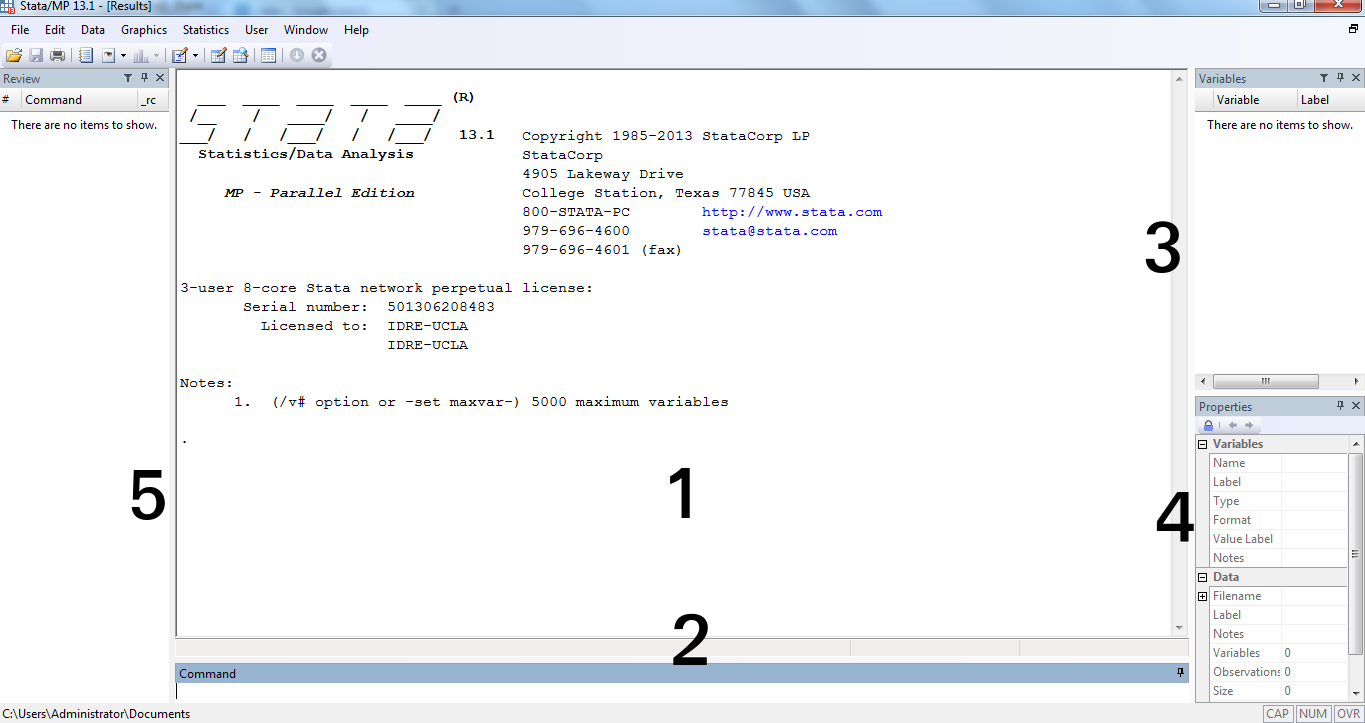
\includegraphics[width=\linewidth]{./img/stata_interface.png}
	\caption{Stata's interface.}
\end{figure}

Upon starting Stata you will see the following sections:

\begin{enumerate}
	\item The results and outputs of your commands will be displayed in the \textbf{results window}.
	\item The \textbf{command window} is where you want to type your commands and send them to Stata by pressing the Enter key.
	\item If you have a dataset loaded its variables will appear in the \textbf{variables pane}.
	\item You can browse the properties of variables in the \textbf{properties pane}.
	\item The \textbf{review pane} lists all the actions you have taken in Stata.  
\end{enumerate}

At the moment you have no data loaded, that is the reason why your variables window is empty. Today you are going to input manually some data on UK universities. You can find these data in the table below.

\begin{table}[H]
	\begin{centering}
		\caption{Some universities in the UK}
	\end{centering}
\bigskip
	\begin{tabular}{r|c|c|c|c|c|c}
		\multicolumn{1}{c|}{\textbf{Name}}                                      & \textbf{Students} & \textbf{Ranking} & \textbf{Location}                                          & \textbf{\begin{tabular}[c]{@{}c@{}}Nobel\\ laureate\end{tabular}} & \textbf{\begin{tabular}[c]{@{}c@{}}Vice\\ chancellor\end{tabular}} & \textbf{Year} \\
		\begin{tabular}[c]{@{}r@{}}Edinburgh\\ University\end{tabular}         & 35258             & 20               & Scotland                                                   & 20                                                                & Male                                                               & 1582          \\ \hline
		\begin{tabular}[c]{@{}r@{}}Napier\\ University\end{tabular}            & 17264             & 64               & Scotland                                                   & 0                                                                 & Female                                                             & 1992          \\ \hline
		\begin{tabular}[c]{@{}r@{}}University\\ of Essex\end{tabular}          & 11939             & 47               & England                                                    & 2                                                                 & Male                                                               & 1965          \\ \hline
		\begin{tabular}[c]{@{}r@{}}University of\\ Cambridge\end{tabular}      & 18271             & 1                & England                                                    & 91                                                                & Male                                                               & 1209          \\ \hline
		\begin{tabular}[c]{@{}r@{}}Cardiff\\ University\end{tabular}           & 30180             & 27               & Wales                                                      & 2                                                                 & Male                                                               & 1997          \\ \hline
		\begin{tabular}[c]{@{}r@{}}University of\\ Liverpool\end{tabular}      & 21276             & 59               & England                                                    & 9                                                                 & Female                                                             & 1903          \\ \hline
		\begin{tabular}[c]{@{}r@{}}Queen's\\ University\\ Belfast\end{tabular} & 24955             & 45               & \begin{tabular}[c]{@{}c@{}}Northern\\ Ireland\end{tabular} & 3                                                                 & Male                                                               & 1908          \\ \hline
		\begin{tabular}[c]{@{}r@{}}Glasgow\\ Caledonian\end{tabular}           & 18410             & 89               & Scotland                                                   & 1                                                                 & Female                                                             & 1993          \\ \hline
		\begin{tabular}[c]{@{}r@{}}Ulster\\ University\end{tabular}            & 26200             & 82               & \begin{tabular}[c]{@{}c@{}}Northern\\ Ireland\end{tabular} & 0                                                                 & Male                                                               & 1982          \\ \hline
		\begin{tabular}[c]{@{}r@{}}University of\\ Warwick\end{tabular}        & 23420             & 6                & England                                                    & 1                                                                 & Male                                                               & 1965         
	\end{tabular}
\end{table}

As you can see there are seven variables and ten observations. You need the following variables:

\begin{itemize}
	\item Name of university.
	\item Total number of students (numeric).
	\item Position in the The Guardian Ranking.
	\item Geographical location (categorical, see below).
	\item Number of affiliated Nobel laureates (numeric).
	\item Gender of the Vice-chancellor (binary, see below).
	\item Year in which it was established (numeric).
\end{itemize}

The variable ``Location'' has the following four categories: Scotland = 1, Northern Ireland = 2, Wales = 3, and England = 4. The variable ``Vice-chancellor'' should be coded as Male = 0 and Female = 1.

You need to think of suitable \textbf{variable names}, \textbf{variable labels}, and \textbf{value labels}. Keep in mind that is customary, but not mandatory, to name variables with small letters. Stata accepts both upper cases and lower cases, but it is case sensitive! Also, variable names cannot contain spaces and the use of underscores is customary when signalising spaces. After thinking of some variable names, open up the data editor by clicking on the icon with a pencil over a spreadsheet (see Figure 2). Stata's data editor resembles very much Excel. Your ``spreadsheet'' should be empty, but if it was not you could type \texttt{clear all} in the command window to get rid of previous data.

\begin{figure}[H]
	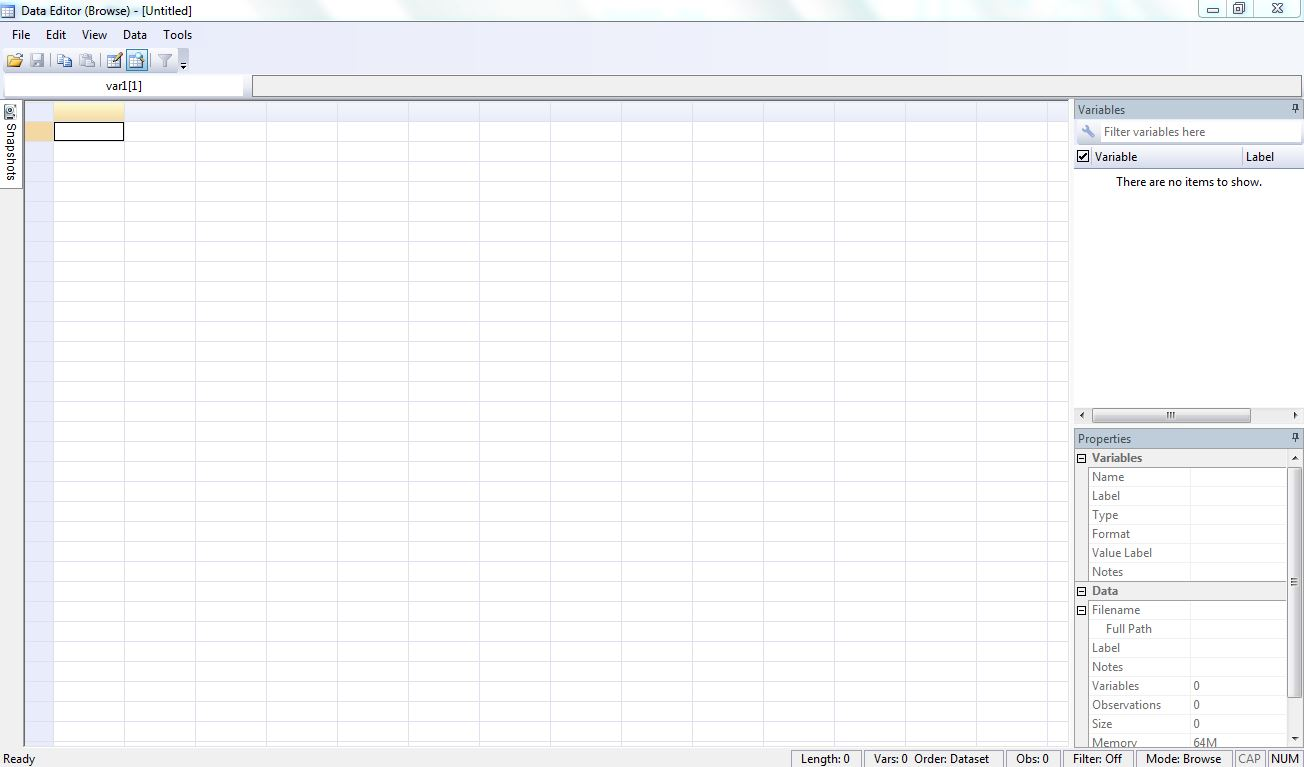
\includegraphics[width=\linewidth]{./img/stata_data_editor_blank.jpg}
	\caption{Stata's data editor.}
\end{figure}

Now it is time to enter the data; start by typing in the first observation (University of Edinburgh). If you press the Tab key you will move onto the next cell. Keep entering the values for all variables for the University of Edinburgh (your first observation). Here it is important to remember that rows represent observations whereas columns represent variables. You might notice that Stata is naming your variables as \textit{var1}, \textit{var2}, and so on. To change \textbf{variable names} simply select a variable in the variables pane (top right corner) and change its name in the properties pane (bottom right corner). Repeat the process for the rest of variables. Let me remind you again that we need a number for geographical location and gender (the categories are specified above).

From the properties pane you can also define \textbf{variable labels}. The process is identical as before: select a variable in the variables pane, switch to the properties pane and give the variable a label (but this time using the box named ``Label''). Variable labels allow spaces. Remember to be precise and accurate with your labelling, but try to keep your labels parsimonious (not too short as to make them ambiguous, but not too long either). Once you have named and labelled your variables you should see the new names and labels in the variables window.

Now that you have assigned names and labels to all your variables, you are going to assign \textbf{value labels} to two variables: geographical location and vice-chancellor (remember the above-mentioned specifications). But first try typing in the command window:

\begin{lstlisting}
	tabulate gender
\end{lstlisting} 

In the command above, \texttt{tabulate} creates a tabulation of a variable named ``gender.'' If you did not name your variable ``gender'', you will have to substitute in your variable's name instead of ``gender.'' In the results window you can see now a table with two categories: 0 and 1. You know that 0 = Male and 1 = Female, but when you report these results you want your readers to know exactly what is going on. Changing 0 to ``Male'' and 1 to ``Female'' is what you do when you assign \textbf{value labels} to your vice-chancellor's gender variable.

\begin{figure}[H]
	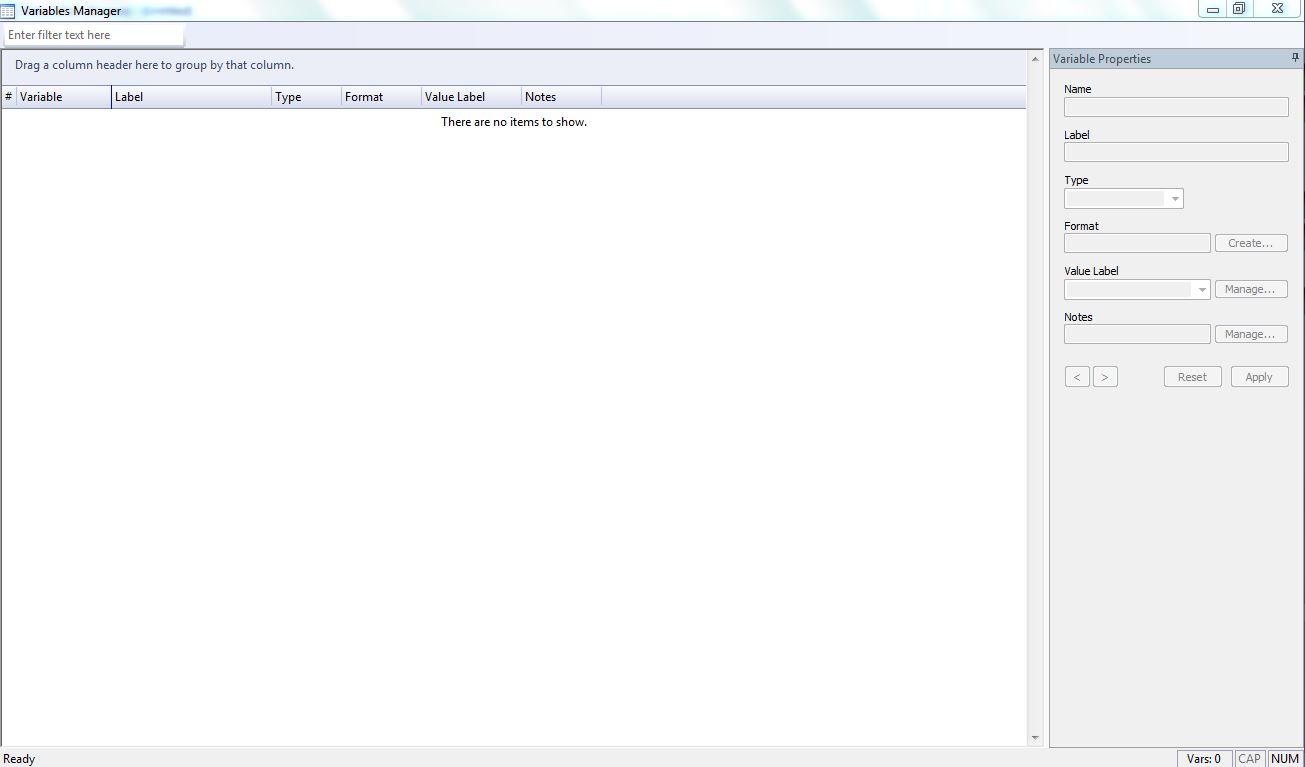
\includegraphics[width=\linewidth]{./img/stata_variables_manager.jpg}
	\caption{Stata's variables manager.}
\end{figure}

To assign value labels you need to exit the data editor and open the \textit{variables manager}. This can be accessed by clicking on the icon with a spreadsheet. Once the variables manager shows up (see Figure 3 for the generic, blank window) you need to create first a set of value labels which you will be attaching to a specific variable later on. Click on \textbf{Manage...} (situated on the right side of the window). In the new window click on \textbf{Create Label}. Yet a new window named \textbf{Create Label} will appear on screen. Give to your new set of value labels a name (in the \textbf{Label name} box). It is best if you name it with something that resembles the name of the variable you are modifying. For example, if you created a variable named ``location'' for the geographical location of universities you can name your set of value labels as ``locationlab'' or ``locationl.'' Keep in mind that sets of value labels cannot use variable names. Now type in the box named \textbf{Value} the original value you gave to your variable (i.e., 0 = Male, so you would type ``0'' here) and in the \textbf{Label} box type its new label (i.e., ``Male''). Then click on \textbf{Add} and repeat the process for 1 = Female. Once this is done click on \textbf{OK}.

Now that you have a set of value labels, the last thing you need to do is attach that set to the original variable. For this, go back to the variables manager window (Figure 3), select the variable at stake, and click on the down arrow located to the right of \textbf{Value Label}. A dropdown menu in which you can select the appropriate set of value labels will appear. Finally, click on \textbf{Apply}. If you use the \texttt{tabulate} command again you will see that your tabulation, this time, reports ``Female'' and ``Male'' instead of 1 and 0. Well done!

%------------------------%------------------------%
% Exercise 3
\setcounter{figure}{0}
\section{\hfil Lab Worksheet III \hfil}
\subsection*{Preparing data}
\addcontentsline{toc}{subsection}{Preparing data}
	
In this exercise you will use some real data. Download from LEARN the dataset named \textbf{essuk12.dta}, which corresponds to the sixth round of the European Social Survey. This dataset has been simplified for today's tutorial's sake and it comprises information on the UK in 2012. Open the dataset with Stata by clicking on \textbf{File$\to$Open} and select \textbf{essuk12.dta}. You should now see some variables listed down in the \textit{variables window} on the right side of your screen.

Today's task is to do some light data management, which entails:

\begin{itemize}
	\item Exploring your dataset,
	\item renaming variables, and
	\item recoding variables.
\end{itemize}

\subsection*{Data exploration}
The command \texttt{\underline{de}scribe}, as its name indicates, describes data in memory or in file. Many commands in Stata can be abbreviated, thus \texttt{describe} can also be used as \texttt{de} (notice how I underlined the shortest abbreviation possible above). You can use this command to describe the entire dataset, or just a selection of variables. For example, if you typed

\begin{lstlisting}
	describe
\end{lstlisting}

you would be describing all variables in the dataset. If you wanted to describe only some variables you could type

\begin{lstlisting}
	de Tvtot Vote Happy
\end{lstlisting}

and describe only those three variables of interest. You can get more information on \texttt{describe} by using another command:

\begin{lstlisting}
	help describe
\end{lstlisting}

The \texttt{help} command opens Stata's manual and shows detailed information on the command you need help with. Remember to consult Stata's manual whenever you are not sure how to use a command. Now try to use \texttt{describe} yourself and answer these questions:

\begin{enumerate}
	\item How many variables are there in the dataset?
	\item How many observations does this dataset have?
	\item What is the difference between ``variable label'' and ``value label''?
\end{enumerate}

Another useful command is \texttt{codebook} (if you type \texttt{help codebook} you will see that it cannot be abbreviated). This one also describes the contents of a dataset, however it provides you with a more detailed description of the data. Just like \texttt{describe}, you can use \texttt{codebook} on the whole dataset or on a selection of variables of interest. Try the following command and answer the questions:

\begin{lstlisting}
	codebook Tvtot Gndr Sclmeet
\end{lstlisting}

\begin{enumerate}
	\item How many response categories does ``Sclmeet'' have?
	\item How is ``Gndr'' coded?
	\item What does ``Tvtot'' measure?
\end{enumerate}

\subsection*{Renaming variables}

When you download a dataset, variables' names not always make sense. Consider the variable ``Sclmeet''; if you use \texttt{describe} and \texttt{codebook} on this variable you can find what it measures. Let's rename the variable to something else, for example ``Socmeet'' (mind the capital -S). To achieve this type the following:

\begin{lstlisting}
	rename Sclmeet Socmeet
\end{lstlisting}

You can use \texttt{help rename} to find out more about the command \texttt{rename} (for instance, it can be abbreviated to \texttt{ren}). Now try to rename the variables in your dataset to the following new names (mind all the capital letters):

\begin{itemize}
	\item Gndr to Gender.
	\item Agea to Age.
	\item Eisced to Education.
	\item Hinctnta to Houseincome.
\end{itemize}

Although not mandatory, it is common to specify variable names with lower cases. Right now all your variables start with a capital letter, so if you wanted to change their names you could use the command \texttt{rename} on each variable and change the first letter only. However, this would take quite a while as you would have to repeat the command twelve times. Stata has a way to deal with problems like this one. Instead of typing the same command twelve times try:

\begin{lstlisting}
	re _all, lower
\end{lstlisting}

Remember that \texttt{re} stands for \texttt{rename}. Above you used \texttt{\_all} to tell Stata that you would like to modify all variables in the dataset. Notice that now there is a comma in the command. That comma tells Stata that you are going to use a \textit{command option} (pretty much all commands in Stata allow for options, you can find more about these options in the help page of each command). The option \texttt{lower} tells Stata that you want only lower cases.

\subsection*{Recoding variables}

Recoding variables is a fundamental part of analysing data. The command \texttt{recode}, as its name indicates, recodes variables in your dataset. Use \texttt{help} to find out more about its syntax. Let's now try to recode the variable ``gender'', remember how it is coded (you can find out by using \texttt{codebook}). You want to get the following:

\begin{itemize}
	\item 0 = Male
	\item 1 = Female
\end{itemize}

To achieve this you need to type:

\begin{lstlisting}
	recode gender (1=0) (2=1), generate(gender2) 
\end{lstlisting}

The command above is telling Stata to recode the variable ``gender'' so the value 1 is now 0 (1=0), and the value 2 is now 1 (2=1). In short, the ``old value'' comes first and then you tell Stata the ``new value.'' However, there is one more thing you need to consider. Recoding variables modifies the data, so it is always a good idea to keep intact the original variable (in this case ``gender''). The command \texttt{recode} allows as a command option another command, in this case the command \texttt{generate} (which can be abbreviated to \texttt{g}, but people usually use it as \texttt{gen}). As you can imagine, \texttt{generate} creates a new variable in your dataset. Above, you recoded the variable ``gender'' and, after recoding it, you created a new variable named ``gender2'' (mind the round brackets).

Now try yourself to recode the variable ``vote'' to (do not forget to generate a new variable):

\begin{itemize}
	\item 1 = Yes
	\item 0 = No
	\item -9 = Everything else
\end{itemize}

Remember that you can use \texttt{codebook} to find out how a variable is currently coded. After recoding the variable you can run \texttt{codebook} again to see how your new codes look like. You will notice that the new coding does not have appropriate value labels, but luckily you know now how to create and assign value labels!

%------------------------%------------------------%
% Exercise 4
\setcounter{figure}{0}
\section{\hfil Lab Worksheet IV \hfil}
\subsection*{Univariate analysis and graphing}
\addcontentsline{toc}{subsection}{Univariate analysis and graphing}

Today we are going to use data from the ESS 2012 again. You can find the dataset on LEARN; make sure you download \textbf{essuk12v2.dta} (notice the ``v2''). In this lab session we are going to do some basic descriptive statistics, including tabulating and graphing. One of the simplest things in data analysis is reporting descriptive statistics and simple graphs that show a single variable. This is what we call \textbf{univariate analysis}, and it is very useful when trying to summarise and describe data (which in in turn helps finding patterns in the data). In Stata there are multiple ways to look at descriptive statistics. Last week you were introduced to two useful commands: \texttt{describe} and \texttt{codebook}. Today you will use one more: \texttt{summarize}. Let’s take a look at it, try typing

\begin{lstlisting}
	summarize
\end{lstlisting} 

and you will see a list of summary statistics for all the variables present in your dataset. This command can be shortened to \texttt{su}, and it allows for a selection of variables like this:

\begin{lstlisting}
	su gender tvtot
\end{lstlisting}

In the example above the command \texttt{summarize} only reports on two variables (``gender'' and ``tvtot''). Notice that the command is \texttt{summarize} and not \texttt{summarise}. This command, as you can see, tells you the number of observations, the mean of the variable, the standard deviation, and the minimum and maximum values a variables takes on. Let's now revise the command \texttt{codebook} with an extra option (remember that \texttt{codebook} cannot be shortened):

\begin{lstlisting}
	codebook gender tvtot, compact
\end{lstlisting}

As you can see, \texttt{codebook, compact} provides you with similar information (but not the same). In this case you get variable labels and unique values. Also notice that the command option follows a comma, which tells Stata that you have decided to use an option. You can try typing the following to see what the option \texttt{compact} really does:

\begin{lstlisting}
	codebook gender tvtot
\end{lstlisting}

The option \texttt{compact} presents you with a shorter report, which you might want if presenting summary statistics to someone else. Remember that you also have the \texttt{describe} command:

\begin{lstlisting}
	de gender tvtot
\end{lstlisting}

Just like the other two commands, you can use \texttt{describe} on the entire dataset or on a selection of variables. The important thing to notice is that these three commands report similar yet different information. Now give these commands a try and find the following information:

\begin{itemize}
	\item The variable labels for all variables in the dataset.
	\item The mean of the variable ``age.''
	\item The mode of the variable ``tvtot.''
	\item The minimum and the maximum values of the variable ``socmeet.''
\end{itemize}

After completing the exercise above you might have noticed that the maximum value of ``socmeet'' is oddly high. The answer has to do with response categories. For example, the ESS codes ``Don't know'' as ``88'' and ``Not available'' as ``999.'' This coding allows you identify these categories easily across variables and treat them as \textbf{missing data}. Different datasets will code these categories in different ways, but it is important to know how these categories are coded before doing data analysis.

\subsection*{Tabulating data}

The command \texttt{tabulate}, which you can shorten to \texttt{tab}, creates one-way or two-way tables of frequencies. The command is followed by one or two variables of your interest, for instance:

\begin{lstlisting}
	tabulate socmeet
\end{lstlisting}

If you were interested in seeing the codes of the response categories you could add a command option to \texttt{tabulate} like in the example below (remember that command options follow a comma):

\begin{lstlisting}
	tab socmeet, nolabel
\end{lstlisting}

The option \texttt{nolabel} removes value labels from the tabulation, and it can be shortened to \texttt{nol}. This option could be useful to see at a glance how a variable is coded (but remember that \texttt{codebook} also shows you this information). Now let's change ``Don't know'' to something else that Stata understands as \textbf{missing values}. The command \texttt{replace} will be handy here:

\begin{lstlisting}
	replace socmeet=.a if socmeet==88
\end{lstlisting}

As you can imagine, \texttt{replace} replaces the content of an existing variable, in this case ``socmeet.'' Notice that in the command above there is an \texttt{if} qualifier. This qualifier is telling Stata to perform an action only on those cases that meet the qualification, which in this case is ``when the variable ``socmeet'' equals 88.'' In other words, the command above is saying something like ``for those observations in which the variable ``socmeet'' is ``88'', replace ``socmeet's'' value ``88'' to ``.a''. The baseline dot before the ``a'' is of paramount importance because that is how Stata recognises missing values. Also notice that Stata distinguishes between ``='' and ``=='' (like many other programming languages). The former (``='') is used as a set equal operator, whereas the latter (``=='') is used to test for equality. You can find more about this topic in the ``Stata Cheatsheet'' on LEARN. Now that you have coded the missing values in the variable ``socmeet'' let's tabulate it again:

\begin{lstlisting}
	tab socmeet
\end{lstlisting}

If you compare this new tabulation to the first one, you will notice that three cases are now missing (i.e., the three cases who responded ``Don't know''). You can check how many missing cases a variable has using the \texttt{missing} option like this:

\begin{lstlisting}
	tab socmeet, missing
\end{lstlisting}  

\forceindent \textbf{?} Now try all this by yourself. Let's look for missing values in the variables ``age'', ``gender'', and ``houseincome.'' If you find missing values change them to something like ``.a'' or ``.b''. Do not forget to use command options like \texttt{nolabel} and \texttt{missing}.

The \texttt{if} qualifier can also be used in the command \texttt{tabulate}. For example, say you want to tabulate the gender of those respondents older than 30:

\begin{lstlisting}
	tab gender if age > 30
\end{lstlisting}
 
 Notice that the variable-target of \texttt{tabulate} is ``gender'' whereas the target of the qualifier \texttt{if} is ``age.'' You can be even more specific with your tabulations, for example:
 
\begin{lstlisting}
	tab gender if age > 30 & age < 50
\end{lstlisting}

Notice that after \texttt{\&} (``and'') you need to specify again the target-variable (in this case ``age''). You can use as many variables as you want. Say you wish to know the gender distribution of those of 20 years of age \textbf{or more} and who voted in the last national election:

\begin{lstlisting}
	tab gender if vote==1 & age >= 20
\end{lstlisting}

\forceindent \textbf{?} Try now to find out how many observations are below the fifth decile in the variable ``hoseincome.''

\subsection*{Graphing data}

Producing graphs is an extremely powerful (and useful) way of examining your data. Stata allows you to produce a great variety of graphs, as well as it allows you to customise them. Let's start by producing a pie chart of the average number of hours watching TV (variable ``tvtot''). Using the menu, go to \textbf{Graphics > Pie chart}. Make sure \textit{Graph by categories} is selected, and where it says \textit{Category variable} select ``tvtot.'' Now click on \textbf{Submit} and you will get a pie chart of the variable ``tvtot.'' In your results-window you can see the command for this action:

\begin{lstlisting}
 graph pie, over(tvtot)
\end{lstlisting}

Let's make the plot a bit more attractive. Go to the \textbf{Slices} tab and select \textit{Customize all slice properties}. Then click on \textit{Slice properties (all)}, tick \textit{Explode slide} and in the drop-down menu select \textit{Automatic}. In the same window, select \textit{Customize all slice labels} and click on \textit{Label properties (all)}. In \textit{Label type} select \textit{Percent}. Now click on \textit{OK} and submit your graph. Stata reports the command for all this clicking and pointing in the results-window. You can use that command to reproduce the exact same graph granted that the variable ``tvtot'' remains the same.

\begin{figure}[H]
	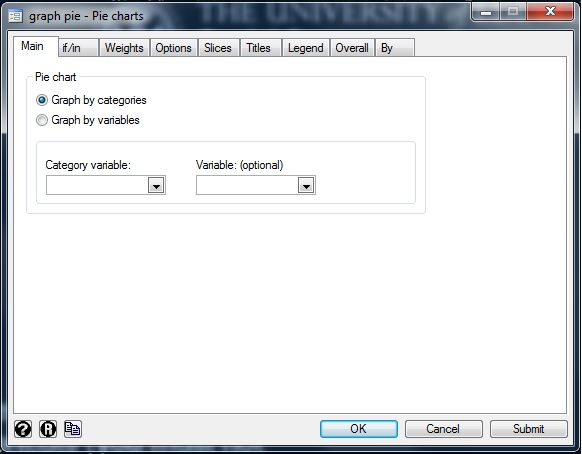
\includegraphics[width=\linewidth]{./img/graphics_pie.jpg}
	\caption{Stata's Graphics > Pie chart.}
\end{figure}

%------------------------%------------------------%
% Exercise 5
\setcounter{figure}{0}
\section{\hfil Lab Worksheet V \hfil}
\subsection*{Bivariate analysis}
\addcontentsline{toc}{subsection}{Bivariate analysis}

Today you will learn how to examine the empirical relationship between two variables in Stata. This examination can be both \textit{descriptive} and \textit{inferential}. There is a number of different ways by which you can achieve this, for instance, cross-tabulations, scatterplots, correlation coefficients, and linear regression. However, whether bivariate analysis is descriptive or inferential will ultimately depend on two things: one is the level of measurement of your variables, and the other is whether you can consider one variable ``\textit{dependent}'' and the other ``\textit{independent}.'' In this exercise we are going to work with categorical variables in the \textbf{essuk12v3.dta} dataset which you can download from LEARN (please mind the ``v3'' in the dataset's name).

\begin{figure}[H]
	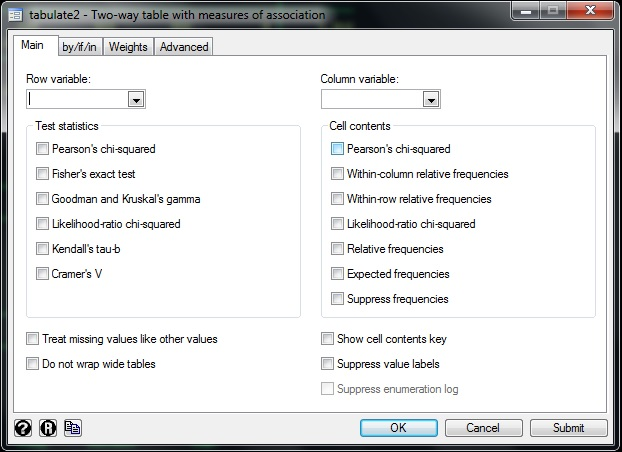
\includegraphics[width=\linewidth]{./img/tabulate2.jpg}
	\caption{Two-way table with measures of association.}
\end{figure}

\subsubsection*{Cross-tabulations}

A \textit{cross-tabulation} is a table with rows and columns in which categorical variables (their frequencies) are represented. These tables are also called ``\textit{contingency tables}'' because the category of a case in one variable is \textit{contingent} on its category in the other variable. For example, the political party a person supports may be contingent on their socio-economic status. If you can identify dependent and independent variables, it is customary to place your dependent variable in columns and your independent variable in rows. Let’s start with a cross-tabulation of whether a person has ever been member of a trade union and their gender. In this example, we are going to assume that whether a person has ever been member of a trade union is more likely if the person is a man (remember that assumptions are given by social theory; numbers are useless without theory!). Here ``gender'' is our independent variable and ``trade union membership'' is our dependent variable.

To get a cross-tabulation of the variables ``gender'' and ``trade union membership'' we can use the command \texttt{tabulate}, but this time we are going to feed in two variables. Alternatively, you can use Stata's menu: go to \textit{Statistics} > \textit{Summaries, tables, and tests} > \textit{Frequency tables} > \textit{Two-way table with measures of association}. You should now see something like Figure 1 above. Select ``gender'' as your \textit{Row variable} and ``union'' as your \textit{Column variable}.Under \textit{Cell contents} tick \textit{Within-row relative frequencies}, this will give you percentages that add up to 100 percent for each row.

\begin{figure}[H]
	\centering
	\resizebox{0.65\textwidth}{!}{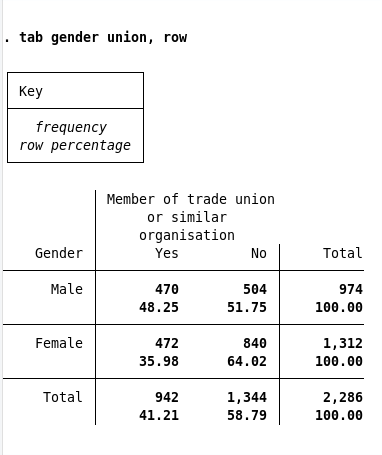
\includegraphics{./img/tab_gender_union_row.png}}
	\caption{Cross-tabulation of gender and union membership.}
\end{figure}

Remember that \texttt{tabulate} can be shortened to \texttt{tab}. The column on the right provides you with the total for each row. The first numbers in each cell of the table are frequencies, whereas the numbers below are percentages. As you can see in Figure 2, there are 974 males in total, 470 of them have ever been member of a trade union. On the other hand, there are 1,312 females in total and 472 of them have ever been member of a trade union. Because each row (i.e., each category of ``gender'') has a different number of observations, it is not easy to compare \textit{absolute frequencies}. It appears that more females have ever been in a trade union, however this is not true when we look at it in \textit{relative terms}. Percentages are greatly useful in cases like this one: in absolute terms, this dataset shows more females that have ever been member of a trade union, but when taking into consideration the number of males and females, it appears that more males, in relative terms, have ever been member of a trade union (48.25 percent versus 35.98 percent). Another important thing to keep in mind is the ``direction'' of the percentages; in this example the proportions have been computed in rows (horizontally), thus you should carry your comparison in columns (vertically).

\subsubsection*{Chi-squared test ($\chi^2$)}

The difference between men and women who have ever been member of a trade union is not very big, but it might be considerable (remember, 48.25 percent versus 35.98 percent). Did we get this difference by \textit{chance}? The sample you are working with is pretty big (2,286 cases), so you may think that there is no reason to think that the difference between men and women is given by chance. Nevertheless, it is good practice to check whether it is \textit{statistically significant}. We can use the chi-squared statistic ($\chi^2$) for examining the likelihood that your results occurred by chance. In simple words, the logic of this test is that if it is extremely unlikely to get this difference between men and women, with such a big sample size, then you can be confident that there was a real difference. However, do not confuse this with the researcher's call to assess whether the difference between men and women is substantially (i.e., theoretically) important.

To perform a chi-squared test in Stata you can use the menu shown in Figure 1, but this time tick \textit{Person's chi-squared} under \textit{Test statistics} and, additionally, you can also tick \textit{Expected frequencies} under \textit{Cell contents}. Alternatively, you can use the following command:

\begin{lstlisting}
	tabulate gender union, row chi2 expected
\end{lstlisting}

The option \texttt{row} gives you percentages in rows, whereas \texttt{chi2} performs the test and \texttt{expected} reports the expected frequencies. These expected frequencies are the number of observations expected if there were no relationship between the two variables in the table. Figure 3 below shows the chi-squared test: you can see that there are 470 men who have ever been member of a trade union (or 48.25 percent of men), but now you also know that you would expect to have 401.4 men here by chance. On the other hand, 472 women have ever been member of a trade union (35.98 percent of women), but you would expect to have 540.6 if the variables were truly independent. In other words, this means that there are $470 – 401.4 = 68.6$ more men that have been member of a trade union than you would expect. At the bottom in Figure 3 you can see the value of Pearson's chi-squared, which is 34.7893 (the number in parenthesis is the degrees of freedom, which is 1 in a 2 by 2 table). The formal way to communicate the results of this test is:

\begin{lstlisting}[escapeinside=**]
*$\chi^2(1, N = 2,286) = 34.7893; p < 0.001$*
\end{lstlisting}

Because $p < 0.001$ (i.e., statistically significant) you can reject the null hypothesis that the two variables are independent. In other words, the data suggest that ``gender'' and ``trade union membership'' are not totally independent. Note that in Figure 3 Stata reports $p = 0.000$. However, this does not mean that the p-value is 0. Stata, in fact, reports an estimate of the probability to three decimal places. Say we got $p = 0.00023$; Stata would round this figure to $p = 0.000$. It is worth-noting that the value $p = 0.00023$ means that you would find this distribution of data only 0.023 percent of the time if the distribution was due to chance.

\begin{figure}[H]
	\centering
	\resizebox{0.7\textwidth}{!}{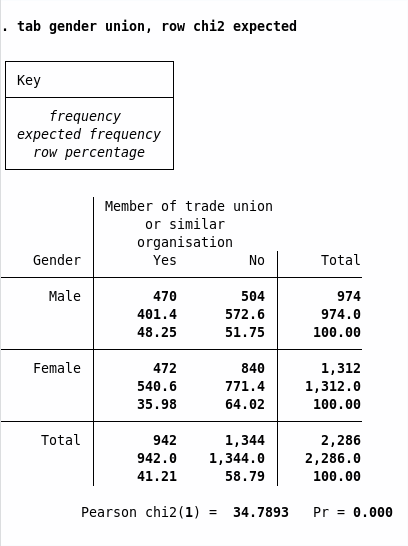
\includegraphics{./img/chi_sq_gender_union.png}}
	\caption{Cross-tabulation of gender and union membership.}
\end{figure}

\noindent\fbox{%
	\parbox{\textwidth}{%
\begin{center}
\textbf{How does the chi-squared test work? (In simple words)}
\end{center}

Pearson's chi-squared test applies to categorical data, and it evaluates how likely it is that an observed distribution of data is due to chance. Sometimes it is also called ``goodness of fit'' statistic because it evaluates how well the observed distribution of data fits the expected distribution if there were no relationship between the variables. Chi-squared is used to test the likelihood that your results \textit{occurred by chance}. This is the reason why we can think of Pearson's chi-squared test as a means to test the null hypothesis that the variables are independent. The test compares the frequency of each cell with the frequency one would expect to obtain were the variables independent. The expected distribution is given by the number of observations in the table's rows and columns. 
    }%
}

\subsubsection*{Measures of association}

\textit{Measures of association} summarise, with a number, the strength of a relationship. Pearson’s chi-squared test is useful in many contexts, but it is not always the best option. A chi-squared test depends greatly on the sample size; this means that the bigger the sample, the bigger chi-squared will be (and you may potentially misinterpret a chi-squared value in big samples, thus concluding that there is a strong relationship between two variables when, in fact, it may be rather weak). To solve this issue, we have two main alternatives: the coefficient phi ($\phi$), and Cramer's V. The way these two work is by simply dividing chi-squared by the maximum value chi-squared itself can be for a given table and a given number of observations (so for a 2 by 2 table this is $N$, and to compute phi we simply calculate the square root of that division. Many people interpret phi as follows:

\begin{itemize}
	\item $0 \geq \phi \leq 0.19$ = weak.
	\item $0.2 \geq \phi \leq 0.49$ = moderate.
	\item $\phi \geq 0.5$ = strong.
\end{itemize}

One thing to keep in mind is that a chi-squared test tells us about statistical significance, whereas measures of association like phi or Cramer's V tell us about the strength of the relationship (that is why the value of phi or V does not change with the sample size). Because phi is used in 2 by 2 tables (and Cramer's V is used for bigger tables), Stata always calculates Cramer's V (you could say one is a special case of the other). To calculate Cramer's V for ``gender'' and ``union membership'' we use the the command option \texttt{V} as shown below:

\begin{lstlisting}
	tabulate gender union, chi2 V
\end{lstlisting}

The result of the command above shows a phi of 0.1234 (remember that phi is for 2 by 2 tables like ours). You can see now that even though chi-squared was statistically significant, phi tells us that the relationship between ``gender'' and ``trade union membership'' is rather weak! Another thing to note is that phi might take on negative values (always from -1 to 1) and Cramer's V goes from 0 to 1.

%------------------------%------------------------%
% Exercise 6
\setcounter{figure}{0}
\section{\hfil Lab Worksheet VI \hfil}
\subsection*{Statistical inference I}
\addcontentsline{toc}{subsection}{Statistical inference I}

This lab worksheet walks you through the very basic concepts of statistical inference (no need for Stata today, pencil and paper will do). For the purposes of this exercise, it will be very helpful if you already know a bit about the following concepts:

\begin{itemize}
    \item Population.
    \item Sample.
    \item Sample statistic.
    \item Sampling distribution.
    \item Central Limit Theorem.
    \item Normal distribution.
\end{itemize}

The main learning goals is to understand what inferential statistic is, but we will also look at how we can collect random samples from larger populations as well as how we go about constructing sampling distributions using repeated random samples. Figure 1 below shows the basic ``statistical procedure.'' As you can see, it has three main components: a \textbf{population} or target group of interest, a \textbf{sample} or sub-group of the target group, and \textbf{probability}, which allows us to say things about the population based on a sample. After collecting a sample, we produce some summaries (i.e., we describe and explore the data). However, this does not really speak of the population but of the observed data in a sample. These observed data might differ from the population, so we rely on probability and inference to draw conclusions. Below Figure 1 there are some questions for you to answer. 

\tikzstyle{population} = [rectangle, rounded corners, minimum width=3cm, minimum height=1cm,text centered, draw=black, fill=red!30]
\tikzstyle{sample} = [trapezium, rounded corners, minimum width=3cm, minimum height=1cm,text centered, draw=black, fill=blue!30]
\tikzstyle{probability} = [circle, minimum width=3cm, minimum height=1cm, text centered, draw=black, fill=green!30]
\tikzstyle{arrow} = [thick,->,>=stealth]

\begin{figure}[H]
\centering
	\begin{tikzpicture}[node distance=4cm]

		\node (pop) [population] {Population};
		\node (samp) [sample, below of=pop] {Sample};
		\node (prob) [probability, right of=samp, xshift=4cm] {Probability};

		\draw [arrow] (pop) -- node[anchor=east]{Data collection} (samp);
		\draw [arrow, dashed] (samp) -- node[anchor=north]{Descriptive statistics} (prob);
		\draw [arrow, dashed] (prob) -- node[anchor=west, xshift=0.2cm]{Statistical inference} (pop);

	\end{tikzpicture}
\caption{Doing statistics.}
\end{figure}

\forceindent \textbf{?} Provide some examples of populations and samples in the box below.

\framebox(347,100){}

\forceindent \textbf{?} Might the following samples (simple random sampling) be representative?

\noindent\fbox{%
	\parbox{\textwidth}{%
		\textbf{Target population:}
		
		Lawyers in Greater London area.
		
		\textbf{Sampling and sample:}
		
		All lawyers working in the Greater London area are assigned an X-digit identification number. 500 lawyers are selected at random by using a random-number generator.
		
		\textbf{How this sample could have been non-representative:}
		
		This samples would not be representative if only lawyers with a British passport had been selected (presumably there are lawyers with non-British passports working in the Greater London area).
	}%
}

\noindent\fbox{%
	\parbox{\textwidth}{%
		\textbf{Target population:}
		
		University students studying in Scotland.
		
		\textbf{Sampling and sample:}
		
		Using Scottish universities' student records, a random sample of 1,000 students was pooled. This sample was designed to comprise students older than eighteen and younger or equal than twenty-four. All nationalities, ethnic groups, and sexes were included. 
		
		\textbf{Is this sample representative? Why/why not? How could it be representative?}
		\newline
		\newline
		\newline
		\newline
	}%
}

\noindent\fbox{%
	\parbox{\textwidth}{%
		\textbf{Target population:}
		
		University students studying in Scotland.
		
		\textbf{Sampling and sample:}
		
		50 interviewers were hired in order to interview university students from all Scottish universities. Interviewers were sent to the field only on odd working calendar-days. Data collection was ended after obtaining 1,000 completed questionnaires.  
		
		\textbf{Is this sample representative? Why/why not? How could it be representative?}
		\newline
		\newline
		\newline
		\newline
	}%
}

\noindent\fbox{%
	\parbox{\textwidth}{%
		\textbf{Target population:}
		
		University students studying in Scotland.
		
		\textbf{Sampling and sample:}
		
		Researchers gather a comprehensive list of university students in Scotland. Students are grouped into ``male'' and``female'' categories. Conveniently, 60 percent of university students in Scotland are female. Therefore, the researchers select at random 600 female students and 400 male students.
		
		\textbf{Is this sample representative? Why/why not? How could it be representative?}
		\newline
		\newline
		\newline
		\newline
	}%
}

Next we are going to construct a sample using simple random sampling. For this, we will use real data from the European Social Survey 2012, but this time we will only focus on respondents from Scotland. On the last page of this worksheet you will find a table with 100 self-reported happiness levels. Happiness was measured from 0 to 10 (being 10 the happiest one can be). Our task is to construct a sample of 15 individuals, so:

\forceindent \textbf{?} What is the value of \textit{N}? And the value of \textit{n}?

\framebox(347,30){}

\forceindent \textbf{?} How would you chose a random sample of 15 individuals from \textit{Table 1}?

\framebox(347,60){}

One ``manual'' way to construct a random sample involves using a table of random numbers. The numbers in the table below were placed in a random order by a computer, so technically is not purely random (but it is good enough for our exercise). We need to use this table of random numbers to chose 15 individuals from \textit{Table 1} that reports happiness levels in Scotland. First we must devise a ``path'' or ``method'', for example: ``two to the right, one down, one left, one up, two left, two up, and repeat'' (it can be easier, of course). Now we place a finger randomly on the table and simply follow our ``path.'' The figure we end up on will be our first sampled individual. Finally we repeat this procedure as many times as necessary.

\forceindent \textbf{?} Annotate below the 15 respondents' ID and their happiness levels.

\framebox(347,47){} 

\noindent\fbox{%
	\parbox{\textwidth}{%
		056 034 074 055 037 064 084 051 050 026 026 078 095 019 073 011 071 017 052 075 052 047 035 071 065 009 077 098 009 002 024 057 059 100 003 021 067 030 087 017 079 091 028 044 024 085 075 077 073 083 054 041 054 013 064 036 067 074 080 064 012 068 027 096 088 066 005 087 069 096 016 083 082 057 031 083 026 050 078 042 076 049 057 006 084 079 067 002 096 040 082 030 041 033 056 062 090 032 034 053 072 062 018 048 084 023 060 049 029 090 007 008 005 015 086 072 086 044 069 068 099 006 011 095 043 073 058 028 093 097 037 092 001 027 047 088 014 089 063 015 058 056 010 074 007 080 088 038 089 010 099 034 028 072 014 061 046 038 061 094 022 063 040 058 003 093 050 053 016 055 065 081 060 021 039 040 037 046 091 004 018 076 001 100 031 038 043 027 075 004 090 059 025 029 069 024 032 059 052 019 045 094 094 047 063 087 041 079 039 085 020 070 020 042 030 065 033 077 046 066 078 070 093 025 054 068 071 089 035 025 081 085 048 060 097 012 092 053 044 045 042 051 022 036 049 081 033 031 062 043 048 032 080 036 095 091 056 034 074 055 037 064 084 051 050 026 026 078 095 019 073 011 071 017 052 075 052 047 035 071 065 009 077 098 009 002 024 057 059 100 003 021 067 030 087 017 079 091 028 044 024 085 075 077 073 083 054 041 054 013 064 036 067 074 080 064 012 068 027 096 088 066 005 087 069 096 016 083 082 057 031 083 026 050 078 042 076 049 057 006 084 079 067 002 096 040 082 030 041 033 056 062 090 032 034 053 072 062 018 048 084 023 060 049 029 090 007 008 005 015 086 072 086 044 069 068 099 006 011 095 043 073 058 028 093 097 037 092 001 027 047 088 014 089 063 015 058 056 010 074 007 080 088 038 089 010 099 034 028 072 014 061 046 038 061 094 022 063 040 058 003 093 050 053 016 055 065 081 060 021 039 040 037 046 091 004 018 076 001 100 031 038 043 027 075 004 090 059 025 029 069 024 032 059 052 019 045 094 094 047 063 087 041 079 039 085 020 070 020 042 030 065 033 077 046 066 078 070 093 025 054 068 071 089 035 025 081 085 048 060 097 012 092 053 044 045 042 051 022 036 049 081 033 031 062 043 048 032 080 036 095 091 056 034 074 055 064 091 011 077 077 052 052 005 021 045 099 037 097 044 078 001 079 074 062 097 091 035 004 024 036 028 051 083 085 027 
	}%
}

We could have calculated the average happiness level using all 100 respondents. However, this would take us more time (although it is easily doable) than sampling 15 individuals and calculating the average happiness. The formula below is how you calculate a mean (use the box below for your computation):

\begin{center}
\scalebox{2}{$\overline{x} = \frac{1}{n} \left(\sum\limits_{i=1}^n x_i\right)$}
\end{center}

\framebox(347,120){} 

With the arithmetic mean you can calculate now the standard deviation as follow:

\begin{center}
	\scalebox{2}{$s = \sqrt{\frac{\sum\limits_{i=1}^n (x_i - \overline{x})^2}{n-1}}$}
\end{center}

\framebox(347,200){} 

In turn, with the standard deviation we can calculate the standard error:

\begin{center}
	\scalebox{2.5}{$s_{\overline{x}} = \frac{s}{\sqrt{n}}$}
\end{center}

\framebox(347,40){} 

Finally we can use the arithmetic mean to create the sampling distribution (of the mean). If we were to repeat the process above 10 times (i.e., if we constructed 10 samples of 15 individuals each) and graph their means (10 means) we would get a graph that might not look ``normally distributed.'' However, if we repeated this 1,000 times the graph will look ``more normal'' (and the more samples you draw, the ``more normal'' your distribution would look like). However, remember that we created a sample of 15 individuals; we probably need a bigger sample size (about 25) to obtain a ``normal'' distribution. There are online applications that recreate this process, but if you have time you can try it yourself ``manually.''

\begin{table}[]
	\centering
	\caption{Happiness in Scotland, 2012}
	\begin{tabular}{cccccc}
		\textbf{ID}                     & \textbf{Happiness} & \textbf{ID}                     & \textbf{Happiness} & \textbf{ID}                   & \textbf{Happiness}            \\
		\textbf{01}                     & 8                  & \textbf{41}                     & 7                  & \textbf{81}                   & 8                             \\
		\textbf{02}                     & 9                  & \textbf{42}                     & 8                  & \textbf{82}                   & 7                             \\
		\textbf{03}                     & 6                  & \textbf{43}                     & 9                  & \textbf{83}                   & 8                             \\
		\textbf{04}                     & 7                  & \textbf{44}                     & 10                 & \textbf{84}                   & 9                             \\
		\textbf{05}                     & 5                  & \textbf{45}                     & 8                  & \textbf{85}                   & 6                             \\
		\textbf{06}                     & 10                 & \textbf{46}                     & 5                  & \textbf{86}                   & 7                             \\
		\textbf{07}                     & 9                  & \textbf{47}                     & 9                  & \textbf{87}                   & 6                             \\
		\textbf{08}                     & 8                  & \textbf{48}                     & 6                  & \textbf{88}                   & 7                             \\
		\textbf{09}                     & 8                  & \textbf{49}                     & 8                  & \textbf{89}                   & 10                            \\
		\textbf{10}                     & 1                  & \textbf{50}                     & 9                  & \textbf{90}                   & 10                            \\
		\multicolumn{1}{l}{\textbf{11}} & 7                  & \multicolumn{1}{l}{\textbf{51}} & 7                  & \textbf{91}                   & 9                             \\
		\multicolumn{1}{l}{\textbf{12}} & 4                  & \multicolumn{1}{l}{\textbf{52}} & 8                  & \textbf{92}                   & 7                             \\
		\multicolumn{1}{l}{\textbf{13}} & 8                  & \multicolumn{1}{l}{\textbf{53}} & 10                 & \textbf{93}                   & 7                             \\
		\multicolumn{1}{l}{\textbf{14}} & 7                  & \multicolumn{1}{l}{\textbf{54}} & 9                  & \textbf{94}                   & 10                            \\
		\multicolumn{1}{l}{\textbf{15}} & 8                  & \multicolumn{1}{l}{\textbf{55}} & 8                  & \textbf{95}                   & 9                             \\
		\multicolumn{1}{l}{\textbf{16}} & 10                 & \multicolumn{1}{l}{\textbf{56}} & 8                  & \textbf{96}                   & 8                             \\
		\multicolumn{1}{l}{\textbf{17}} & 8                  & \multicolumn{1}{l}{\textbf{57}} & 9                  & \textbf{97}                   & 8                             \\
		\multicolumn{1}{l}{\textbf{18}} & 8                  & \multicolumn{1}{l}{\textbf{58}} & 9                  & \textbf{98}                   & 5                             \\
		\multicolumn{1}{l}{\textbf{19}} & 9                  & \multicolumn{1}{l}{\textbf{59}} & 8                  & \textbf{99}                   & 8                             \\
		\multicolumn{1}{l}{\textbf{20}} & 8                  & \multicolumn{1}{l}{\textbf{60}} & 7                  & \textbf{100}                  & 8                             \\
		\multicolumn{1}{l}{\textbf{21}} & 9                  & \multicolumn{1}{l}{\textbf{61}} & 9                  & \multicolumn{1}{l}{\textbf{}} & \multicolumn{1}{l}{\textbf{}} \\
		\multicolumn{1}{l}{\textbf{22}} & 9                  & \multicolumn{1}{l}{\textbf{62}} & 10                 & \multicolumn{1}{l}{\textbf{}} & \multicolumn{1}{l}{\textbf{}} \\
		\textbf{23}                     & 8                  & \textbf{63}                     & 7                  &                               &                               \\
		\textbf{24}                     & 8                  & \textbf{64}                     & 8                  &                               &                               \\
		\textbf{25}                     & 8                  & \textbf{65}                     & 9                  &                               &                               \\
		\textbf{26}                     & 8                  & \textbf{66}                     & 10                 &                               &                               \\
		\textbf{27}                     & 9                  & \textbf{67}                     & 9                  &                               &                               \\
		\textbf{28}                     & 10                 & \textbf{68}                     & 10                 &                               &                               \\
		\textbf{29}                     & 8                  & \textbf{69}                     & 9                  &                               &                               \\
		\textbf{30}                     & 9                  & \textbf{70}                     & 8                  &                               &                               \\
		\textbf{31}                     & 7                  & \textbf{71}                     & 6                  &                               &                               \\
		\textbf{32}                     & 9                  & \textbf{72}                     & 10                 &                               &                               \\
		\textbf{33}                     & 8                  & \textbf{73}                     & 10                 &                               &                               \\
		\textbf{34}                     & 9                  & \textbf{74}                     & 8                  &                               &                               \\
		\textbf{35}                     & 4                  & \textbf{75}                     & 10                 &                               &                               \\
		\textbf{36}                     & 8                  & \textbf{76}                     & 10                 &                               &                               \\
		\textbf{37}                     & 7                  & \textbf{77}                     & 8                  &                               &                               \\
		\textbf{38}                     & 9                  & \textbf{78}                     & 8                  &                               &                               \\
		\textbf{39}                     & 6                  & \textbf{79}                     & 9                  &                               &                               \\
		\textbf{40}                     & 7                  & \textbf{80}                     & 5                  &                               &                              
	\end{tabular}
\end{table}

%------------------------%------------------------%
% Exercise 7
\setcounter{figure}{0}
\section{\hfil Lab Worksheet VII \hfil}
\subsection*{Statistical inference II}
\addcontentsline{toc}{subsection}{Statistical inference II}

This worksheet revises the concepts that you already know about statistical inference (if you need a reminder check \textit{Lab Worksheet VI: Statistical inference I} and the pertinent lecture-slides). You will not need to use Stata for the exercises below. All exercises start with a question mark. 

\forceindent \textbf{?} When is a mean (average) a statistic, and when is it a parameter?

\framebox(347,90){}

\forceindent \textbf{?} If you were constructing a simple random sample from a comprehensive population of 10,000 individuals, how would be your sample's mean distribution \textbf{in terms of normality} if you were to select 50, 1,000, or 2,000 individuals from that population?

\framebox(347,90){}

\forceindent \textbf{?} Can you name the following formulas?

\begin{center}
	\scalebox{2}{$s = \sqrt{\frac{\sum\limits_{i=1}^n (x_i - \overline{x})^2}{n-1}}$}
\end{center}

\begin{center}
	\scalebox{2}{$\overline{x} = \frac{1}{n} \left(\sum\limits_{i=1}^n x_i\right)$}
\end{center}

\begin{center}
	\scalebox{2.5}{$s_{\overline{x}} = \frac{s}{\sqrt{n}}$}
\end{center}

\forceindent \textbf{?} Can you complete the blank spaces in the figure below?

\begin{figure}[H]
	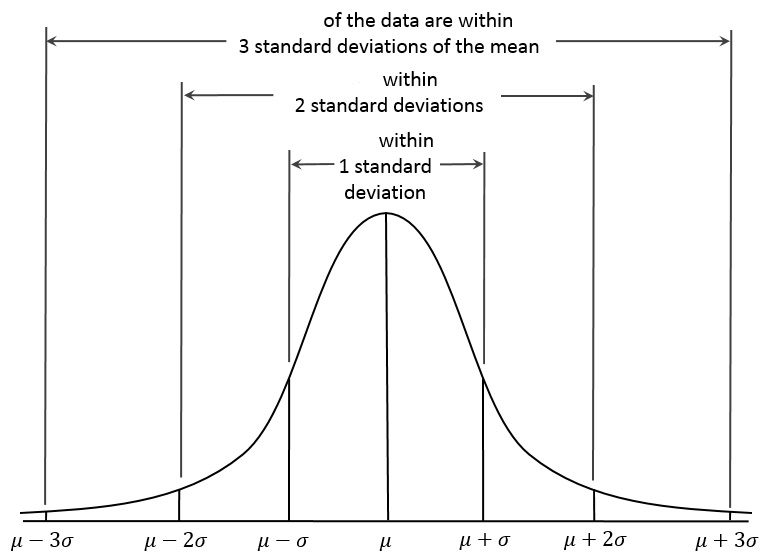
\includegraphics[width=\linewidth]{./img/gaussian_distribution.jpg}
\end{figure}

\forceindent \textbf{?} How is the distribution depicted above called? What theorem makes it useful for data analysis?

\framebox(347,50){}

\forceindent \textbf{?} A simple random sample of students has a mean age of 25 and \textit{n}=500. Can you calculate the standard error with the information provided? If not, what are you missing?

\framebox(347,50){}

\forceindent \textbf{?} A random sample of 100 students did an IQ test. The resulting average IQ was of 106 with a standard deviation of 16. Can you find a 95 percent confidence interval? (Use the formula below).

\begin{center}
	\scalebox{2}{$\overline{x} \pm Z_{\alpha/2}\times\frac{s}{\sqrt{n}}$}
\end{center}

You can use the above formula to compute any confidence interval. The suffix $\alpha$ (alpha) denotes the confidence level. $Z_{\alpha/2}$ is the critical level for a given alpha. Remember that a critical level of a 95 percent confidence interval is about 1.96. For a 95 percent confidence interval the value of alpha is of 0.05 (because $1-0.95=0.05$). Using this information try to calculate the confidence interval for the exercise above.

\framebox(347,130){}

\forceindent \textbf{?} Can you complete the table below?

\begin{table}[H]
	\centering
	\begin{large}
	\begin{tabular}{ccc}
		\underline{$Z_{\alpha/2}$} & \underline{$\alpha$} & \underline{$1-\alpha$} \\
		1.645          & 0.1          &           \\
		1.96          & 0.05          &           \\
		2.576         &          & 0.99        
	\end{tabular}
	\end{large}
\end{table}

\forceindent \textbf{?} The coffee machine of your university's cafeteria is set up in such way that the average content of a cup of coffee equals a quantity $\mu$. Who knows why but you decided to construct a random sample of 200 cups of coffee. This resulted in an average content of 34cl. Assume your standard deviation was of 6cl. Can you find two confidence intervals one for 90 percent and another for 99 percent?

\framebox(347,150){}

%------------------------%------------------------%
% Exercise 8
\setcounter{figure}{0}
\section{\hfil Lab Worksheet VIII \hfil}
\subsection*{Simple regression analysis}
\addcontentsline{toc}{subsection}{Simple regression analysis}

This lab worksheet guides you through the basics of doing simple regression analysis in Stata. The exercise does not really teach you the theory behind regression analysis, instead it focuses on the technical aspect of doing with Stata what you learned in your lectures. If you feel you need a reminder you can look up in the course's materials what regression analysis, regression coefficients, and $R^2$ are. It is also fundamental to know the difference between dependent and independent variables (the latter are also called \textit{predictors} or \textit{regressors}).

The data we are going to use come from the European Social Survey Round 8 (2016) in Great Britain. The dataset is called \textbf{essuk16} and you can find it on LEARN. As we already know, the first step when dealing with new data is to explore them. Use the following commands to find out more about this dataset:

\begin{lstlisting}
	describe
	summarize
	codebook, compact
\end{lstlisting}

These commands are helpful because they tell us things like what the dataset's variable labels mean. Tabulations are useful when exploring data too. Let's see how the data are distributed (remember you can shorten most Stata commands):

\begin{lstlisting}
	tabulate happy
	tabulate trstprt
	tabulate trstplt
	tabulate atchctr
\end{lstlisting}

From the above we want to see things like ``a happiness of 8 out of 10 seems to be the most frequent (about 30 percent)'' or that ``about 60 percent of the British population trust their political parties 4 out of 10 or less.'' We can obtain information from individual variables by using tabulations, but we could also graph the same data:

\begin{lstlisting}
	graph bar (percent), over(trstprt, label(angle(45)))
\end{lstlisting}

The way we explore new datasets partially depends on personal preference, however it ultimately comes down to ``what we need to do'' with the data (perhaps a barplot is more useful if we need to communicate these data to an audience that is not very familiar with tabulations).

Now that you know a bit more about this new dataset, we are going to perform a simple regression analysis. For the sake of this exercise we are going to assume that the following hypothesis is true: \textit{``How happy a person is impacts on their trust in political parties.''} We should also consider a few more things:

\begin{itemize}
	\item If our theory poses that the happier a person is the more trust they will have in political parties, we can expect a positive regression coefficient.
	\item If our theory poses that the happier a person is the less trust they will have in political parties, we can expect a negative regression coefficient.
	\item To verify the points above we need to know how our variables are coded (i.e., ``do they go from least to most?'')
\end{itemize}

We should acknowledge a final note; the two variables we are going to use in our regression analysis are scales, which technically are not continuous but ordered-categorical. Some authors argue that these data can be used in linear regression insofar some assumptions are met. These assumptions are well beyond the scope of this exercise, so we are going to ignore them for simplicity's sake.

To run a simple regression model we type the following in Stata:

\begin{lstlisting}
	regress trstprt happy
\end{lstlisting}

The command \texttt{regress} can be shortened to \texttt{reg}. Remember that you can find out more about any Stata command with the command \texttt{help}. The first variable in our regression command represents our \textit{dependent variable}, whilst the rest of variables (in this case there is only one) are our \textit{independent variables}. In other words, we are assessing the impact of happiness on trust in political parties. Figure 1 below shows the regression output.

\begin{figure}[H]
	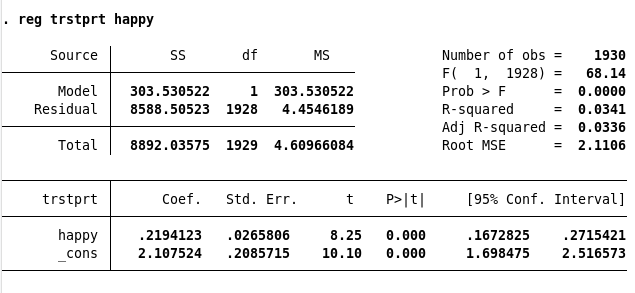
\includegraphics[width=\linewidth]{./img/reg1.png}
	\caption{Simple linear regression with happiness as predictor.}
\end{figure}

We can see that this model was performed on 1,930 respondents (why do you think the model missed 29 people?) The value of $R^2$ is not impressive (a mere 0.034). This figure indicates that 3.4 percent of the variance in our dependent variable (trust in political parties) is explained by the model (which has only one predictor, happiness). The regression coefficient of happiness is statistically significant at the 0.001 level, but the impact seems rather small: for each one-unit increase in happiness we can expect about 0.22 increase in trust. The constant is statistically significant too, and it indicates the value of the dependent variable when all independent variables are zero (in other words, if we were to graph the regression line the constant is the point at which the line would cut the vertical Y-axis). According to this model, our ``starting point'' is of about 2 points of trust.

Perhaps happiness is not the best ``predictor'' of trust in political parties. Let's use this time trust in politicians as a predictor of trust in political parties. We could assume the following (rather redundant) hypothesis: ``people with high levels of trust in politicians will also show high levels of trust in political parties.''

\begin{lstlisting}
	regress trstprt trstplt
\end{lstlisting}

\begin{figure}[H]
	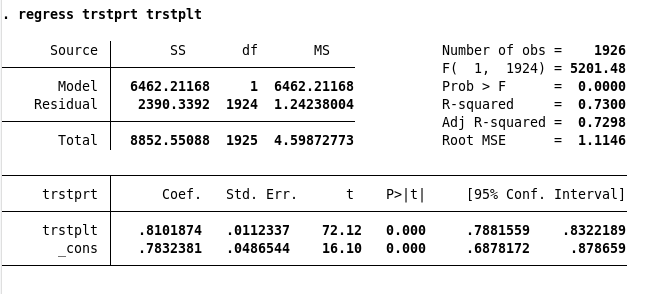
\includegraphics[width=\linewidth]{./img/reg2.png}
	\caption{Simple linear regression with trust in politicians as predictor.}
\end{figure}

We can see several changes. First, the number of observations went down to 1,926. On the other hand, $R^2$ went up drastically to 0.73 (73 percent of the variance in our dependent variable is explained by our model). The value of $R^2$ is very high, and in this case it might be a sign that our variables are really measuring the same thing. The regression coefficient is again statistically significant at the 0.001 level (so we can say with confidence that is different from zero). The coefficient itself predicts an increase of 0.81 in trust in political parties for each unit-increase in trust in politicians, i.e., when trust in politicians increase by 1 we can expect an increase in trust in parties of 0.81. Because both variables are measured using the same scale we can easily see that the change is pretty similar (but not identical).

Let's run one last regression. This time we are going to predict happiness using the age of our respondents. Our research question could well be either ``older people are happier than younger people'' or the opposite.

\begin{lstlisting}
	regress happy agea
\end{lstlisting}

\begin{figure}[H]
	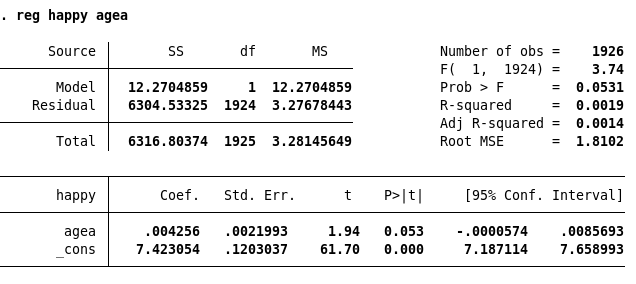
\includegraphics[width=\linewidth]{./img/reg3.png}
	\caption{Simple linear regression with age as a predictor of happiness.}
\end{figure}

Notice the value of $R^2$ (0.0019). According to this model, age accounts for a mere 0.19 percent of the variance (information) in happiness. We can also see that the coefficient is not statistically significant at the 0.05 level (yet just so). The coefficient itself would suggest that a one-unit increase in age results in about 0.0043 increase in happiness. This model is not very useful as it does not explain the variance of our dependent variable very well. Exploring the data before and after performing an analysis is critical to finding issues with the distribution of the data that might account for poor-performing models. For example, we could have plotted the average of happiness for each age to see if there is a pattern:

\begin{lstlisting}
graph bar (mean) happy, over(agea, label(labsize(tiny) angle(45)))
\end{lstlisting}

The resulting graph does not show a clear pattern, and more importantly it does not suggest any linearity at all (remember the ``linear'' in ``linear regression''). Keep in mind that when doing ``real'' linear regression analysis (i.e., not a lab exercise) the technique requires some important assumptions to be true.

%------------------------%------------------------%
% Exercise 9
\setcounter{figure}{0}
\section{\hfil Lab Worksheet IX \hfil}
\subsection*{Multiple regression analysis}
\addcontentsline{toc}{subsection}{Multiple regression analysis}

In today's worksheet we are going to do some multiple regression analysis on respondents' self-reported happiness using the \textit{European Social Survey}. You can find the dataset \textbf{essuk16.dta} on LEARN. Since it is the same dataset we used in the previous worksheet, the same caveats established then also apply here (e.g., regression assumptions are not considered for simplicity's sake) . Remember three key Stata commands widely used to explore datasets:

\begin{lstlisting}
	describe
	summarize
	codebook, compact
\end{lstlisting}

We should be paying attention to things like the number of variables in the dataset, what they measure, how they are coded, whether we have missing cases and how these are coded. Last time we focused on the variables ``happy'', ``trstprt'', ``trstplt'', and ``atchctr.'' This time let's try:

\begin{lstlisting}
tabulate agea
tabulate region
tabulate gender
\end{lstlisting}

From the first tabulation we can see that respondents' ages range from 15 to 94. The command \texttt{summarize} would have given us this information more easily:

\begin{lstlisting}
summarize agea
\end{lstlisting}

However, remember that tabulations are not always the best way to represent and explore data. Since ``agea'' is a continuous variable we could plot it in a histogram:

\begin{lstlisting}
histogram agea, frequency
\end{lstlisting}

Also, you can explore two variables at the same time using the command \texttt{histogram}. For example, we could plot the distribution of respondents' ages in each region:

\begin{lstlisting}
histogram agea, frequency by(region)
\end{lstlisting}

On the other hand, ``region'' is a categorical variable, so we could plot it with bars like this:

\begin{lstlisting}
graph bar (percent), over(region, label(angle(45)))
\end{lstlisting}

The variable ``gndr'' is also categorical; however if you try plotting it in a bar chart or pie chart you might find it redundant because the variable only has two categories. Perhaps it is more convenient representing ``gndr'' with a simple tabulation (but again, this is a matter of personal preference). Stata allows you to explore data in a myriad of ways. For instance, consider the following:

\begin{lstlisting}
table gndr, contents(freq mean agea) row
\end{lstlisting}

With the \texttt{table} command and the \texttt{contents} option we can explore gender and age at the same time. The tabulation above shows the mean (average) age for males and females. Tabulating means (not only frequencies or percentages) could sometimes be very useful. If you were to ask the data ``are males happier than females?'' you would probably want to start by looking at the average level of happiness:

\begin{lstlisting}
table gndr, contents(freq mean happy) row
\end{lstlisting}

and you would find that female respondents are ever so slightly happier than male respondents on average (7.66 versus 7.6).

Now that we have explored a few variables let's run some regressions. Start with:

\begin{lstlisting}
regress happy gndr agea ib7.region
\end{lstlisting}

\begin{figure}[H]
	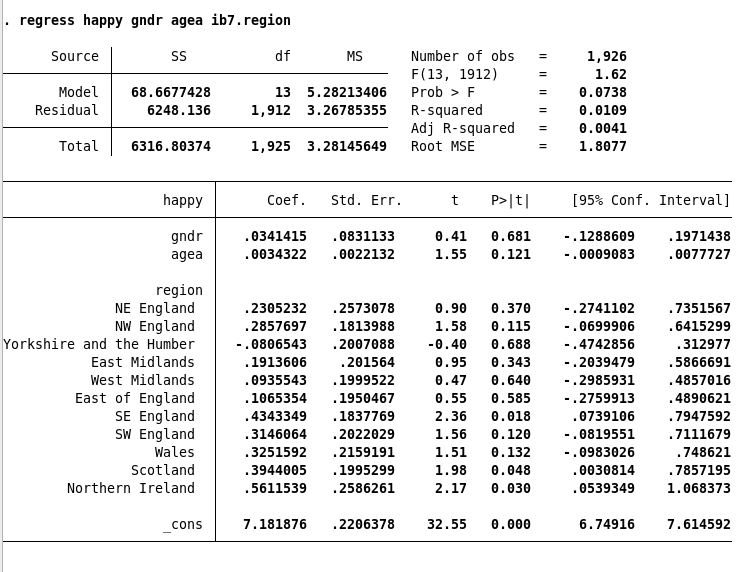
\includegraphics[width=\linewidth]{./img/mult_reg1.png}
	\caption{Multiple linear regression model with happiness as outcome.}
\end{figure}

Remember that linear regression requires continuous variables as your dependent variable. In the model above, variables ``happy'' and ``agea'' are considered continuous, whereas ``gndr'' and ``region'' are categorical. It is important to tell Stata that it needs to treat specific variables as categorical, for your model will need $X-1$ \textit{dummy variables} (where $X$ is the total number of categories in a variable). Take ``region'' as an example: this variables has twelve categories (twelve regions), therefore your model will need eleven dummy variables and one \textit{base group}. In the command above, Stata has been instructed to treat ``London'' as base group (\texttt{ib7.} does that, if you wanted the second category to be the base group instead, you can type \texttt{ib2.} before the variable name).

The value of $R^2$ tells you the proportion of variance in your dependent variable (``happy'') that is explained by the model. In this case, we can see that this model does not really explain much, only 1.1 percent of variance or information. Moreover, if we look at the $p$-value for the $F$-test of overall significance (reported as $Prob > F$ in Stata) we can see that it is not statistically significant itself. This is telling us that our model does not fit any better than a model with no predictors (also called \textit{intercept-only}). 

Most coefficients are not statistically significant at the 0.05 level (we already knew this from the $F$-test of overall significance). A non-statistically significant coefficient is telling you that we cannot be sure the coefficient (i.e., the value of the parameter) is actually different from zero. If you look at the confidence interval of a non-statistically significant coefficient, you will see that the interval includes zero in its range. This means you should not interpret that coefficient. However, do acknowledge in your papers and reports that you have non-statistically significant coefficients by simply saying so.

Let's now run the following regression model:

\begin{lstlisting}
regress atcherp gndr agea ib7.region
\end{lstlisting}

Notice that this new model loses 16 observations (not many) when compared to our previous ``happiness model'' (the observations go from 1,926 to 1,910). However, now our $F$-test is statistically significant  ($Prob > F = 0.0000$), meaning that our model fits better than an empty or intercept-only model. The model explains about 2.8 percent of information in the dependent variable ``atcherp'' (a 0-to-10 scale of emotional attachment to Europe).

It is of \underline{paramount importance} to bear in mind that the interpretation of coefficients of categorical variables is \underline{totally different} from the interpretation of coefficients of continuous variables. Below the coefficients of the variables ``agea'' (continuous) and ``gndr'' (categorical) are interpreted for you:

\begin{itemize}
	\item ``agea'': keeping the rest of variables constant, for each one-unit increase in a respondent's age we expect a decrease of 0.01 points in emotional attachment to Europe.
	\item ``gndr'': keeping the rest of variables constant, female respondents present an emotional attachment to Europe 0.281 points higher than that of male respondents. 
\end{itemize}

\begin{figure}[H]
	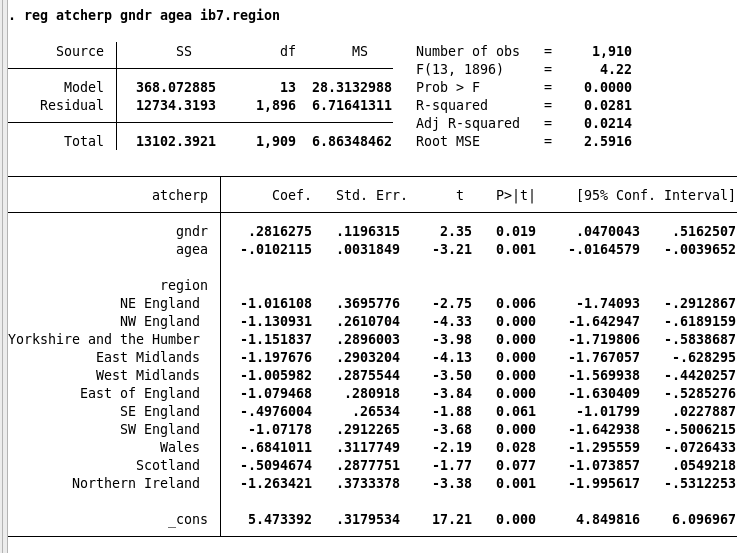
\includegraphics[width=\linewidth]{./img/mult_reg2.png}
	\caption{Multiple linear regression model with emotional attachment to Europe as outcome.}
\end{figure}

Firstly, notice that when interpreting regression coefficients in multiple regression \textit{you must} keep constant the variables you are not interpreting. Secondly, when interpreting continuous variables we speak of ``one-unit increase'' if the coefficient is positive or of ``one-unit decrease'' if the coefficient is negative. However, when interpreting categorical variables (dummy variables) we compare groups to the base group. In the example above, there are only two categories: males and females. Because the variable is coded 1 "male'' and 2 ``female'', Stata takes by default the first value, ``male'', as base group. The coefficient of ``gndr'', therefore, is really the coefficient of female respondents in comparison to that of male respondents. Here too a positive coefficient means an increase, but it is an increase over the base group's effect on the dependent variable. To clarify this point further consider the variable ``region'' below (remember the base group was ``London''):

\begin{itemize}
	\item ``NE England'': keeping the rest of variables constant, respondents from the North East (England) are 1 point less emotionally attached to Europe than respondents from London.
	\item ``Scotland'': keeping the rest of variables constant, respondents from Scotland are 0.51 points less emotionally attached to Europe than respondents from London.
\end{itemize}

Because all regional categories (i.e., all the dummy variables in the model) present a negative coefficient, we know that London is the region most emotionally attached to Europe. The interpretation of all these coefficients will therefore be in ``negative'' terms (less than the base group). Needless to say that if we did not know that ``London'' is the base group we could not interpret these figures. Also, notice that Scotland's coefficient is not statistically significant. What you already know about statistical significance also applies here in the same fashion: because $p > 0.05$ in the case of the category ``Scotland'', we cannot say for sure the coefficient is different for zero (and we do not interpret it). Finally, the closer the coefficient of a dummy variable is to zero the more similar that category is to the base group.   
%------------------------%------------------------%

\end{document}
